
\section{Symmetric Cryptography}

\paragraph{One-time pad}
Plaintext $p$, key $k$ such that $|p| = |k|$.
Ciphertext $c = p \xor k$.

If $k$ u.a.r. and only used once then the OTP is \textbf{perfectly secure}, i.e.
$ \Pr[P=p|C=c] = \Pr[P=p]$.

Note: keys can re-occur (as a result of random sampling) but they must not be re-used (i.e. the adversary must not be aware that the same key is used).

Issues: same lengths, key distribution, single use.

\subsection{Block Ciphers}

\paragraph{Block cipher}
A block cipher with key length $k$ and block size $n$ consists of two efficiently computable permutations\footnote{Encipher and decipher}:
$$ E: \setzeroone^k \times \setzeroone^n \mapsto \setzeroone^n \quad
D: \setzeroone^k \times \setzeroone^n \mapsto \setzeroone^n $$
such that for all keys $K$ $D_K$ is the inverse of $E_K$
(where we write $E_K$ short for $E(K, \cdot)$).

\paragraph{Security notions}
Known plaintext attack, chosen plaintext attack, chosen ciphertext attack.
Exhaustive key search on $(P,C)$ pairs -- no attack should be better, else we throw the cipher away.

\paragraph{Pseudo-randomness}
\begin{itemize}
\item Adversary $\A$ interacts either with block cipher $(E_K, D_K)$ or a truly random permutation $(\Pi, \Pi^{-1})$.
\item A block cipher is called a \textbf{pseudo-random permutation PRP} if no efficient\footnote{Quantified by runtime + number of oracle queries.} $\A$ can tell the difference between $E_K$ and $\Pi$ (no access to the inverse).
\item A block cipher is called a \textbf{strong-PRP} if no efficient $\A$ can tell the difference between $(E_K, D_K)$ and $(\Pi, \Pi^{-1})$.
\end{itemize}

\begin{figure}[h]
    \centering
	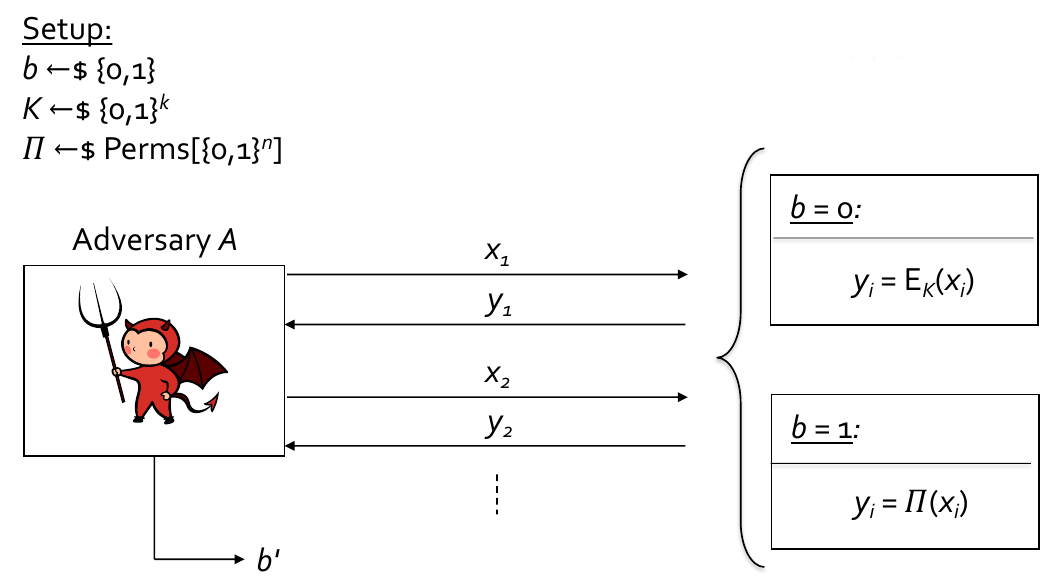
\includegraphics[scale=0.4]{images/prp.png}
    \caption{PRP game}
    \label{fig:prp}
\end{figure}

The advantage is defined as:
$$
\mathbf{Adv}^{PRP}_E (\A)
= 2 \cdot \Big| \Pr[ \text{Game }\textbf{PRP}(\A, E) \Rightarrow \text{true} ] - \frac{1}{2} \Big|
$$
where the probability is over the randomness of $b, K, \Pi, \A$.
Note that:
$$
\Pr[ \text{Game }\textbf{PRP}(\A, E) \Rightarrow \text{true} ]
= \Pr[b'=b]
$$
Also see the Advantage Rewriting Lemma (\ref{adv-rewr-lemm}).

\paragraph{Constructing block ciphers}
In general: keyed round function that is repeated many times.

\begin{itemize}
\item Feistel cipher: halved blocks crossing back and forth, e.g. DES
\item Substitution-permutation network: confusion + diffusion, e.g. AES
\end{itemize}

\paragraph{Electronic Code Book (ECB) mode}
Same plaintext always maps to the same ciphertext (deterministic).
Thus serious leakage, don't use.

\begin{figure}[h]
    \centering
	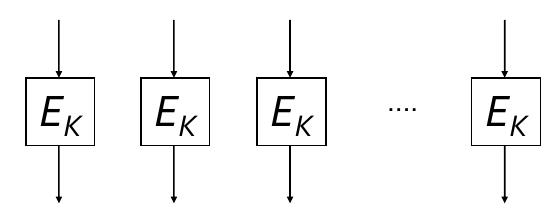
\includegraphics[scale=0.4]{images/ecb.png}
    \caption{ECB mode}
    \label{fig:ecb}
\end{figure}

\paragraph{Cipher Block Chaining (CBC) mode}
Use u.a.r. IV/previous ciphertext block to randomise encryption.

A bit flip in $C_i$ completely scrambles/randomises $P_i$ and flips the same bit in $P_{i+1}$.

Caveats: non-random IV, padding oracle attack, ciphertext block collisions (after using the same key for $2^{n/2}$ blocks by the birthday bound).

\begin{figure}[h]
    \centering
	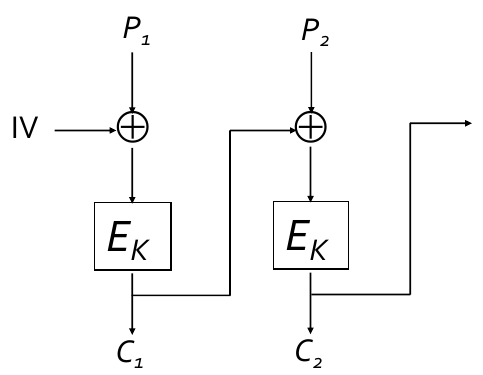
\includegraphics[scale=0.4]{images/cbc-enc.png}
	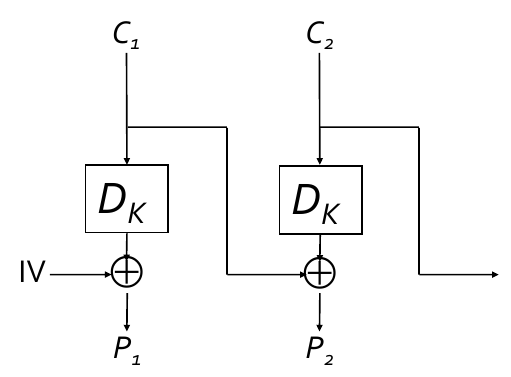
\includegraphics[scale=0.4]{images/cbc-dec.png}
    \caption{CBC mode (left: encipher, right: decipher)}
    \label{fig:cbc}
\end{figure}

\paragraph{Counter (CTR) mode}
Incrementing counter is encrypted with block cipher to produce a pseudo-random value to xor the plaintext block with.

Effectively a stream cipher producing OTP keys.
$E_K$ does not even need to be invertible.
No padding needed, can just truncate the last block.
A bit flip it $C_i$ flips the same bit in $P_i$.

Caveats: counter must not repeat/wrap around (else xor of ciphertexts = xor of plaintexts).

\begin{figure}[h]
    \centering
	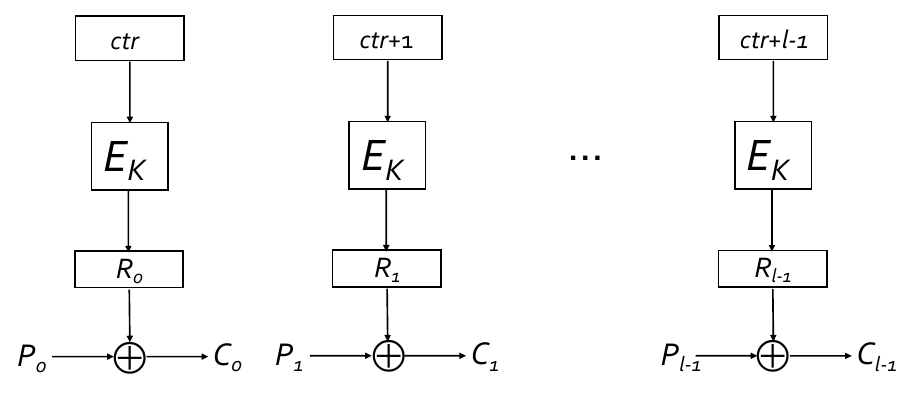
\includegraphics[scale=0.4]{images/ctr.png}
    \caption{CTR mode}
    \label{fig:ctr}
\end{figure}



\subsection{Symmetric Encryption}

\paragraph{Symmetric Encryption Scheme}
is a triple $ SE = (KGen, Enc, Dec) $.
We have key space $\K = \setzeroone^k$, message space $\M = \setzeroone^*$\footnote{In reality we might have a maximum plaintext length.} and ciphertext space $\C = \setzeroone^*$.
For correctness, we have $ Dec_K(Enc_K(m))=m $.

\paragraph{IND-CPA Security}
Informally:
computational version of perfect security --
an efficient adversary cannot compute anything useful from a ciphertext (e.g. hide every bit of the plaintext).
Equivalent to \emph{semantic security}.

Formally:
For any efficient adversary $\A$, given the encryption of one of two equal-length messages of its choice,
$\A$ is unable to distinguish which one of the two messages was encrypted.

In the security game, $\A$ gets access to a \emph{Left-or-Right encryption oracle}.
The advantage of $\A$ is:
$$
\adv^{IND-CPA}_{SE} (\A)
= 2 \cdot \Big| \Pr[ \text{Game }\textbf{IND-CPA}(\A, SE) \Rightarrow \text{true} ] - \frac{1}{2} \Big|
$$

Notes:
Deterministic schemes \textbf{cannot} be IND-CPA secure (why?\footnote{The adversary can first query $(m_0, m_0)$ to learn $c_0$, then query $(m_0, m_1)$ and thus win with high probability.}).
CBC and CTR mode (if used properly) can be proven to be IND-CPA secure (assuming that $Enc$ is a PRP-secure block cipher).

Caveats:
No integrity. Says nothing about messages of non-equal length. No chosen ciphertexts.

\begin{figure}[h]
    \centering
	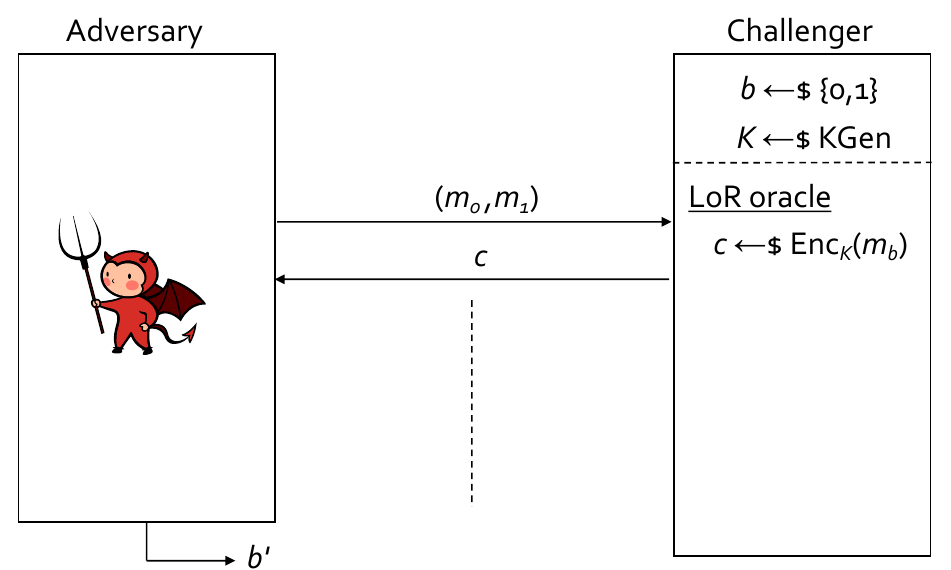
\includegraphics[scale=0.4]{images/ind-cpa.png}
    \caption{IND-CPA game}
    \label{fig:ind-cpa}
\end{figure}

\paragraph{Advantage Rewriting Lemma}\label{adv-rewr-lemm}
Let $b$ be a uniformly random bit and $b'$ the output of some algorithm. Then:
\begin{align*}
2 \Big| \Pr[b'=b] - \frac{1}{2} \Big|
&= \Big| \Pr[b'=1|b=1] - \Pr[b'=1|b=0] \Big| \\
&= \Big| \Pr[b'=0|b=0] - \Pr[b'=0|b=1] \Big|
\end{align*}

\paragraph{Difference Lemma}
Let $Z, W_1, W_2$ be events. If
$$
(W_1 \wedge \neg Z) \text{ occurs if and only if } (W_2 \wedge \neg Z) \text{ occurs}
$$
then
$$
\Big| \Pr[W_2] - \Pr[W_1] \Big| \leq \Pr[Z]
$$
In practice: $Z$ is a bad event that rarely happens, $W_1, W_2$ are when $\A$ wins in security games $G_1, G_2$.
Useful for \emph{game hopping} proofs.

\paragraph{PRP-PRF Switching Lemma}
Let $E$ be a block cipher.
Then for any algorithm $\A$ making $q$ queries:
$$
\Big| \adv^{PRP}_{E} (\A) - \adv^{PRF}_{E} (\A) \Big| \leq \frac{q^2}{2^{n+1}}
$$



\subsection{Attacks}

\paragraph{Padding}
Added before encryption to expand plaintext to a multiple of the block size, i.e. \\$pad(\cdot): \setzeroone^* \mapsto \{ \setzeroone^n \}^*$.
Must be expanding (why?) and efficiently computable.
May be either randomised or deterministic.
\\
E.g. TLS padding: appends $t+1$ bytes of value $t$.

Problem: adversary can detect padding errors (explicit error messages, logs, timing differences).

\paragraph{Padding Oracle}
Given a ciphertext $C$, returns whether the padding of the decryption is valid or invalid.
Leaks 1 bit of information.
Kind of a chosen ciphertext attack, thus \underline{not} covered by IND-CPA security!
Main problem: no ciphertext integrity.

In practice:
$\A$ needs 128 oracle queries on average to recover one plaintext byte.
Repeat for all bytes and all blocks for full plaintext recovery.
Additional practical details to consider.
For TLS attacks, see Lucky 13 and POODLE.

\begin{figure}[h]
    \centering
	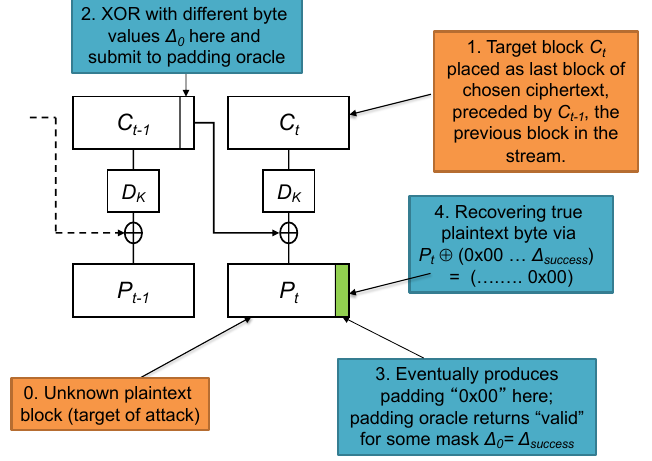
\includegraphics[scale=0.6]{images/cbc-padding-oracle-attack.png}
    \caption{Padding oracle attack on CBC mode}
    \label{fig:cbc-padding-oracle-attack}
\end{figure}

\paragraph{Predictable IVs}
Random IVs are not just theoretically relevant for IND-CPA security of CBC mode.
Consider the following steps (see \autoref{fig:cbc-predictable-iv}):
\begin{enumerate}
\item $\A$ queries LoR oracle with $(P_0, P_1)$
\item Oracle responds with $C = C_0||C_1$ where $C_1 = E_K(P_b \xor C_0)$
\item $\A$ predicts next $IV=C_0'$
\item $\A$ queries $P_0 \xor C_0 \xor C_0'$
\item $\implies b = 0 \iff P_b = P_0 \iff C_1 = C_1' \implies$ breaks IND-CPA security
\end{enumerate}

In practice: systems may use \emph{IV chaining} (use the last ciphertext as the next IV, in order to avoid having to sample new randomness).
E.g.: SSLv3, TLS 1.0, SSH in CBC mode.
See also the BEAST attack on TLS.

\begin{figure}[h]
    \centering
	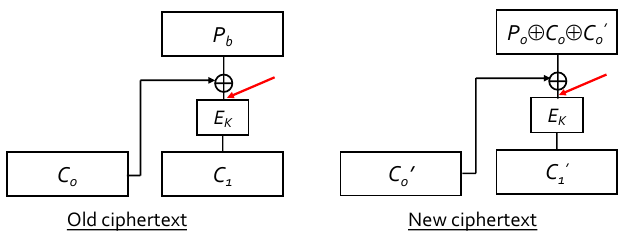
\includegraphics[scale=0.6]{images/cbc-predictable-iv.png}
    \caption{Attack on predictable IVs in CBC mode}
    \label{fig:cbc-predictable-iv}
\end{figure}



\subsection{Hash Functions}

\paragraph{Cryptographic Hash Function}
An efficiently computable function $H: \setzeroone^* \mapsto \setzeroone^n$ that maps arbitrary-length inputs to fixed-length outputs (``\emph{message digests}'').
Not keyed!

Applications: MACs, signatures, key derivation, commitments.

\paragraph{Random oracle model}
Model under which hash functions are assumed to produced outputs that are uniformly random distributed.
I.e. a hash function could be modelled by a random oracle.
Very strong assumption!

\paragraph{Birthday paradox}
When drawing elements at random from a set of size $s$ then after $\sqrt{s}$ trials we expect a collision with 39\% probability.
We quickly get to 99\% with an additional constant factor.

\paragraph{Security goals}
Primary goals:
\begin{itemize}
	\item \emph{Pre-image resistance} (one-wayness):
	Given $h$, it is infeasible to find an $m$ such that $H(m) = h$.
	\item \emph{Second pre-image resistance}:
	Given $m_1$, it is infeasible to find an $m_2$ such that $H(m_1) = H(m_2)$.
	\item \emph{Collision resistance}:
	It is infeasible to find any $m_1 \neq m_2$ such that $H(m_1) = H(m_2)$.
\end{itemize}

Secondary goals:
\begin{itemize}
	\item \emph{Near-collision resistance}:
	It is infeasible to find any $m_1 \neq m_2$ such that $H(m_1) \approx H(m_2)$ (e.g. hashes agree on most bits).
	\item \emph{Partial pre-image resistance 1}:
	Given $H(m)$, it is infeasible to recover any partial information about $m$.
	\item \emph{Partial pre-image resistance 2}:
	Given a target string $t$ with $|t|=l$ it is infeasible to find an $m$ such $H(m)=t||x$ (faster than with $2^l$ brute-force hash evaluations).
\end{itemize}

CR adversary:\\
Cannot quantify security over \underline{all} efficient $\A$ (collisions exist, $\A$ can hardcode one).
Instead, define ``$(t, \varepsilon)$-CR adversaries'', running in time $t$ and with $\adv^{CR}_H(\A) = \varepsilon$.
Build reductions from there.

Relationships:
\begin{itemize}
\item Collision resistance $\implies$ second pre-image resistance
\item Maybe: Collision resistance $\implies$ pre-image resistance -- depending on how you define pre-image resistance (sampling from the domain or from the range?)
\end{itemize}

Generic attacks (in the ROM):\\
(Second) pre-image resistance: $2^n$ evaluations.\\
Collision resistance: $2^{n/2}$ evaluations! (by the birthday paradox)\\
$\implies$ e.g. SHA-1 with 160-bit outputs only achieves 80-bit security

\paragraph{Merkle-Damgård iterated hashing}
Constructs a hash function $H$ from a \emph{compression function} \mbox{$h: \setzeroone^k \times \setzeroone^n \mapsto \setzeroone^n$}.
Used e.g. in MD5, SHA-1, SHA-2.

Steps: pad message, split into k-bit chunks, repeatedly apply $h$ to the chunks and IV/chaining values (see \autoref{fig:merkle-damgard}).

Padding scheme:
$$ m' = pad(m) = m || 10^t || [len(m)]_k $$
where $[len(m)]_k$ is the k-bit encoding of the message length\footnote{This limits the maximum length of a message that can be hashed to $2^k - 1$.}
and $0 \leq t < k$ is minimal.

Theorem: If $h$ is collision resistant, then so is $H$.%
\footnote{Note that the choice of padding scheme matters for the proof!
Also note that the two IVs must be the same for a \emph{full collision}.
The much weaker form of two colliding messages for different IVs is called a \emph{freestart collision}.}

Length extension attack:
Given $H(m)$ (but not $m$!) once can compute a valid hash $y=H(pad(m)||m'')$.
This is problematic e.g. when construction MACs or KDFs from a hash function.

\begin{figure}[h]
    \centering
	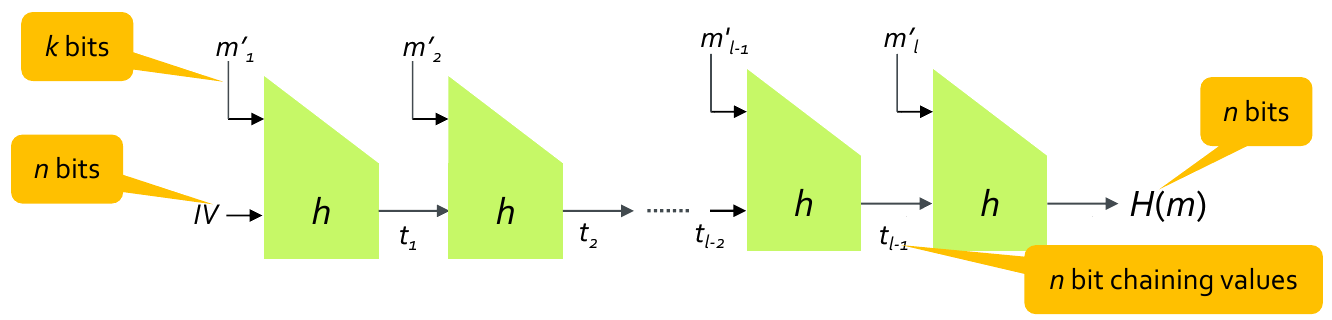
\includegraphics[scale=0.4]{images/merkle-damgard.png}
    \caption{Merkle-Damgård transform}
    \label{fig:merkle-damgard}
\end{figure}

\paragraph{Constructing compression functions from block ciphers}
E.g. Davies-Meyer, Matyas-Meyer-Oseas, Miyaguchi-Preneel constructions.
Use message as the key (need fast rekeying!) and (some variation of) chaining value as ``plaintext'' input.

\begin{figure}[h]
    \centering
	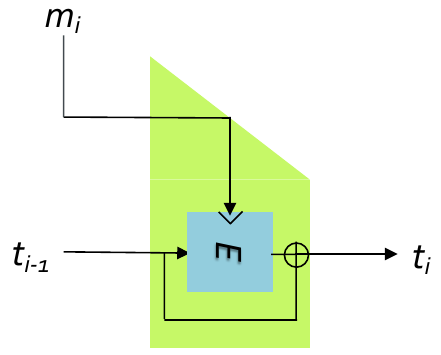
\includegraphics[scale=0.35]{images/davies-meyer.png}
    \caption{Davies-Meyer construction}
    \label{fig:davies-meyer}
\end{figure}

\paragraph{Sponge construction}
Different design approach.
Centered around 2 phases: absorbing + squeezing.
Key ideas: giant bit permutation $F$, not inputting/outputting entire state.
Variable length output.

E.g. used in SHA-3/Keccak: $\text{SHA-3}(m)=out_1||out_2||out_3||...$.

\begin{figure}[h]
    \centering
	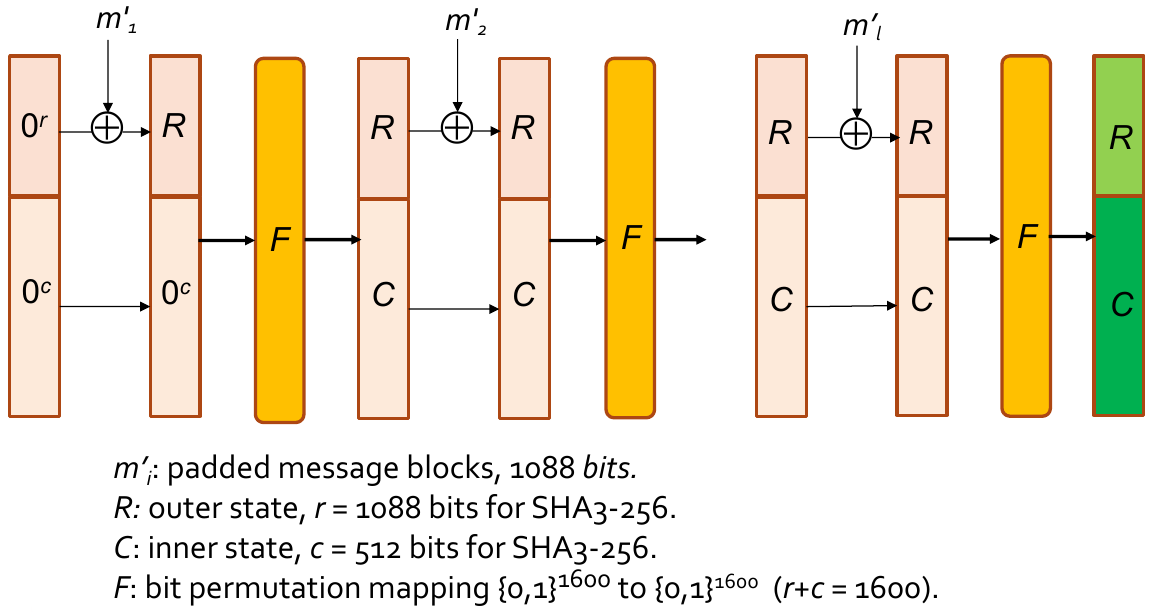
\includegraphics[scale=0.35]{images/sponge-absorb.png}
    \caption{Sponge construction: absorbing}
    \label{fig:sponge-absorb}
\end{figure}
\begin{figure}[h]
    \centering
	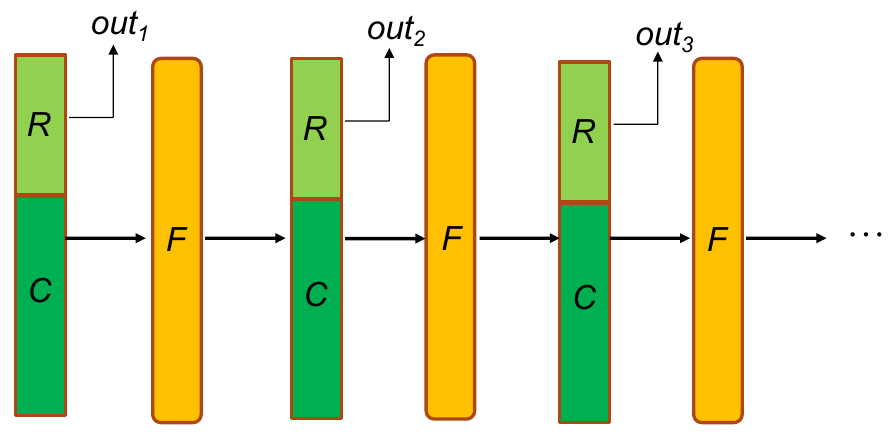
\includegraphics[scale=0.35]{images/sponge-squeeze.png}
    \caption{Sponge construction: squeezing}
    \label{fig:sponge-squeeze}
\end{figure}



\subsection{Message Authentication Codes MACs}

\paragraph{Motivation}
Provide \emph{integrity} and \emph{data origin authentication}, i.e. no attacker should be able to modify or forge messages (unforgeability).

They do \underline{not} provide confidentiality or secure against message deletion, replay, reordering, or reflection (if the key is used in both directions).

\paragraph{Definition (MAC scheme)}
A MAC scheme with key length $k$ and tag length $t$ consists of three efficient algorithms:
\begin{align*}
KGen:& \quad \{\} \mapsto \setzeroone^k \\
Tag:& \quad \setzeroone^k \times \setzeroone^* \mapsto \setzeroone^t \\
Vfy:& \quad \setzeroone^k \times \setzeroone^* \times \setzeroone^t \mapsto \setzeroone
\end{align*}
For correctness\footnote{A functionality, not a security requirement.}, we require that
$$
\forall K, m \; . \; Vfy(K, M, \tau) = 1 \text{ where } \tau = Tag(K,m)
$$
$Vfy$ and $Tag$ may be randomised.
Note that if they are deterministic \underline{and} $Vfy$ internally (re)computes $Tag(K, m) \overset{?}{=} \tau$, then the scheme has \emph{unique tags}.

\paragraph{MAC Security}
Informally: it is hard for an attacker to forge a valid message-tag pair $(m', \tau')$.

Security game: $\A$ gets access to a tag oracle and a verify oracle.

\begin{figure}[h]
    \centering
	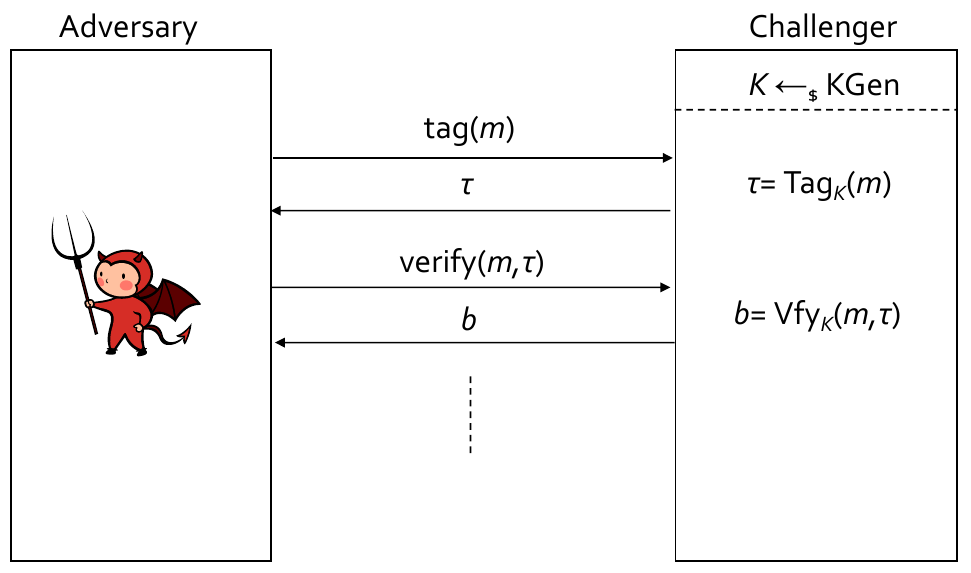
\includegraphics[scale=0.35]{images/mac.png}
    \caption{MAC game}
    \label{fig:mac}
\end{figure}

\paragraph{Weak unforgeability under chosen message attack (WUF-CMA)}
$\A$ wins if it submitted some $(m^*, \tau^*)$ to the verify oracle such that $Vfy(m^*, \tau^*)=1$ and \underline{no} query $Tag(m^*)$ was made.

\paragraph{Strong unforgeability under chosen message attack (SUF-CMA)}
$\A$ wins if it submitted some $(m^*, \tau^*)$ to the verify oracle such that $Vfy(m^*, \tau^*)=1$ and \underline{no} query $Tag(m^*)$ \underline{with response} $\tau^*$ was made.

Note that:
\begin{itemize}
\item A SUF-CMA adversary can \underline{also} win by coming up with a new tag for an old message.
We make the adversary ``stronger'' by relaxing the winning condition.
\item SUF-CMA $\implies$ WUF-CMA (somewhat counter-intuitively)
\item For deterministic MAC schemes \underline{that build $Vfy$ from $Tag$}, the two are equal (why?%
\footnote{When tags are unique then no adversary can come up with another tag for a previously queried message.
However, consider the following deterministic scheme that is WUF-CMA but not SUF-CMA:
$$ Tag'(K, m) = 0 || Tag(K, m) \quad Vfy'(K, m, b||\tau) = Vfy(K, m, \tau)$$
}).
\item More formally: $(q_t, q_v, t, \varepsilon)$-W/SUF-CMA security
\end{itemize}

Generic attacks:
guess $(m, \tau)$ pairs, guess the key, few tag queries + exhaustive key search.

\paragraph{MACs from PRFs}
Construction of $MAC(F)$:
Let $F: \setzeroone^k \times \setzeroone^n \mapsto \setzeroone^t$ be a PRF.
\begin{align*}
KGen():& \quad K \leftarrow \$ \; \setzeroone^k \\
Tag(K, m):& \quad \tau \leftarrow F(K, m) \\
Vfy(K, m, \tau):& \quad \tau' \leftarrow F(K, m); \text{ return } \tau' == \tau
\end{align*}
%
Theorem:
If $F$ is a PRF then $MAC(F)$ is a SUF-CMA.

\paragraph{Domain extension with CR hashing}
Motivation: build a MAC for a larger input domain $\mathcal{X}'$ from a MAC with fixed domain $\mathcal{X}$ (to handle more than just block-sized messages).

Construction of $HtMAC$:
Let $MAC=(KGen, Tag, Vfy)$ be a MAC and let $H: \mathcal{X}' \mapsto \mathcal{X}$ be a hash function.
\begin{align*}
Tag'(K, m):& \quad Tag(K, H(m)) \\
Vfy'(K, m, \tau):& \quad Vfy(K, H(m), \tau)
\end{align*}
%
Theorem:
If $MAC$ is SUF-CMA secure and $H$ is collision resistant then $HtMAC$ is SUF-CMA.

\paragraph{Hash-based MAC HMAC}
Turn (the often fast) hash functions into a keyed primitive using a two-key nest to build a PRF (and thus a MAC):
$$
F_{nest}((K_1, K_2), m) = H(K_2 || H(K_1||m))
$$
Notes:
Cannot simply prepend the key (length extension attacks).
Also cannot simply append the key (offline collision attacks).
In practice, derive two keys from one key using an inner and outer mask.
Implementations often use an initialise-update-finalise interface (which can open \href{https://eprint.iacr.org/2015/1129}{timing attack vectors}).

HMAC is gradually supplanted by faster designs based on universal hashing (see below), yet it is still used in key derivation scenarios (that use PRFness).

\begin{figure}[h]
    \centering
	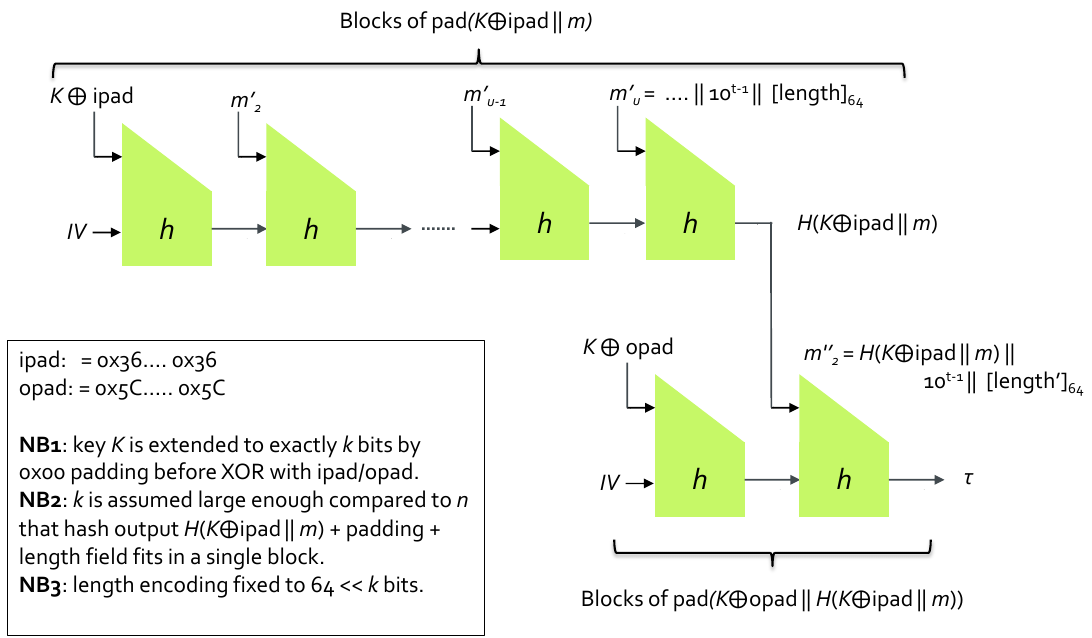
\includegraphics[scale=0.45]{images/hmac.png}
    \caption{HMAC}
    \label{fig:hmac}
\end{figure}

\paragraph{Nonce}
A number used once.
Does neither need to be secret, nor does it need to be unpredictable.
But must never ever repeat.
Reasoning: it is easier to only use a number once than it is to get a good source of randomness.

\paragraph{Nonce-based MAC NMAC}
Like normal MAC, but $Tag$ and $Vfy$ now also take a nonce $N \in \mathcal{N}$.
In the security game, we require that nonces are distinct (e.g. enforced by the tag oracle).

\paragraph{Keyed hash function}
A keyed hash function $H$ is a deterministic algorithm that takes a key and a message and produces a \emph{digest} $t=H(K, m)$ over the digest space $\mathcal{T}$.

\paragraph{Universal hashing UHF}
Informally: selecting a hash function at random from a family of hash functions (the universal family).

Security game:
Let $H$ be a \underline{keyed} hash function. Then:
\begin{enumerate}
\item Challenger sets $K \leftarrow \$ \; \setzeroone^k$
\item Adversary outputs distinct $(m_0, m_1)$
\end{enumerate}
$\A$ wins if $H(K, m_0) = H(K, m_1)$ and has advantage $\adv^{UHF}_{H}(\A)$.

$H$ is an $\varepsilon$-\emph{bounded universal hash function} if $\adv^{UHF}_{H}(\A) \leq \varepsilon$ for all $\A$ (even unbounded ones).

Equivalent definition:
$H$ is an $\varepsilon$-UHF if
$ \forall m_0, m_1 \; . \; \Pr[H(K, m_0) = H(K, m_1)] \leq \varepsilon $,
where the probability is over the random choice of $K$.

\paragraph{Universal hash functions from polynomials}
Let $\mathcal{F}$ be a finite field (e.g. integers mod p or $GF(2^n)$)
and let $\mathcal{K} = \mathcal{T} = \mathcal{F}$ and $\mathcal{M} = \mathcal{F}^{\leq l}$.
Then we define:
$$
H_{poly}(K, (a_1, \dots, a_v))
= K^v + a_1 K^{v-1} + a_2 K^{v-2} + \dots + a_{v-1} K + a_v
$$
That is, $H_{poly}$ is always a degree $v$ polynomial (even if the message vector $a$ is zero).
It can efficiently be evaluated using finite field operations and Horner's rule.

Theorem:
$H_{poly}$ is an $\varepsilon$-UHF for $\varepsilon = \frac{l}{|\mathcal{F}|}$.

\paragraph{Difference unpredictable hashing DUHF}
Security game:
Let $H$ be a keyed hash function and let the digest space $\mathcal{T}$ have a group operation $+$ (with inverse $-$)%
\footnote{E.g. addition mod $n$ in $\mathbb{Z}_n$ or XOR in $\setzeroone^n$.}.
Then:
\begin{enumerate}
\item Challenger sets $K \leftarrow \$ \; \setzeroone^k$
\item Adversary outputs distinct $m_0, m_1 \in \mathcal{M}$ and $\delta \in \mathcal{T}$.
\end{enumerate}
$\A$ wins if $H(K, m_0) - H(K, m_1) = \delta$ and has advantage $\adv^{DUHF}_{H}(\A)$.

$H$ is an $\varepsilon$-\emph{bounded distance unpredictable hash function} ($\varepsilon$-DUHF) if $\adv^{DUHF}_{H}(\A) \leq \varepsilon$ for all $\A$ (even unbounded ones).

\paragraph{XOR universal hashing}
Special case of DUHF where we have XOR as the group operation.
We define $H_{xpoly}$ as follows:
\begin{align*}
H_{xpoly}(K, (a_1, \dots, a_v))
&= K^{v+1} + a_1 K^v + a_2 K^{v-1} + \dots + a_{v-1} K^2 + a_v K \\
&= K \cdot H_{poly}(K, (a_1, \dots, a_v))
\end{align*}

Theorem:
$H_{xpoly}$ is an $\varepsilon$-DUHF for $\varepsilon = \frac{l+1}{|\mathcal{F}|}$.

\paragraph{Carter-Wegman MACs}
Let $H$ be an $\varepsilon$-DUHF and let $F$ be a PRF.
Then we define CW-MAC$(F, H)$ as follows:
\begin{align*}
KGen():& \quad (K_1, K_2) \leftarrow \$ \; \mathcal{K}_H \times \mathcal{K}_F \\
Tag((K_1, K_2), N, m):& \quad \tau \leftarrow H(K_1, m) + F(K_2, N) \\
Vfy((K_1, K_2), N, m, \tau):& \quad \tau' \leftarrow Tag((K_1, K_2), N, m); \text{ return } \tau' == \tau
\end{align*}

Theorem:
If $H$ is an $\varepsilon$-DUHF and $F$ a PRF then CW-MAC$(F, H)$ is SUF-CMA secure.

In practice: e.g. GMAC (used in AES-GCM) instantiates $F$ with AES and $H$ with $H_{xpoly}$ over $\mathcal{F} = GF(2^{128})$.

\begin{figure}[h]
    \centering
	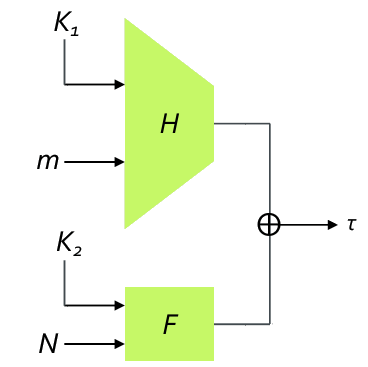
\includegraphics[scale=0.45]{images/carter-wegman.png}
    \caption{Carter-Wegman MAC tag algorithm}
    \label{fig:carter-wegman}
\end{figure}



\subsection{Authenticated Encryption}

\paragraph{Integrity of ciphertexts INT-CTXT}
Informally: adversary cannot forge new ciphertexts.

Security game:
$\A$ can submit any $m$ to an encryption oracle to obtain $c=Enc_K(m)$.
At the end $\A$ submits one $c^*$ to a $try$ oracle.

$\A$ wins if 1) $c^*$ is distinct from all previously seen $c$ and 2) $c^*$ decrypts to a $m^* \neq \bot$.

$\A$ has advantage $\adv^{INT-CTXT}_{SE}(\A)$.

\paragraph{Integrity of plaintexts INT-PTXT}
Informally: adversary cannot force a new plaintext to be accepted by the receiver.

Same as INT-CTXT but with an additional winning requirement: \\
$\A$ wins if \dots\ 3) $m^*$ is distinct from all previous queries $m$.

INT-CTXT $\implies$ INT-PTXT\footnote{Since due to SE correctness a new plaintext implies a new ciphertext.}

\begin{figure}[h]
    \centering
	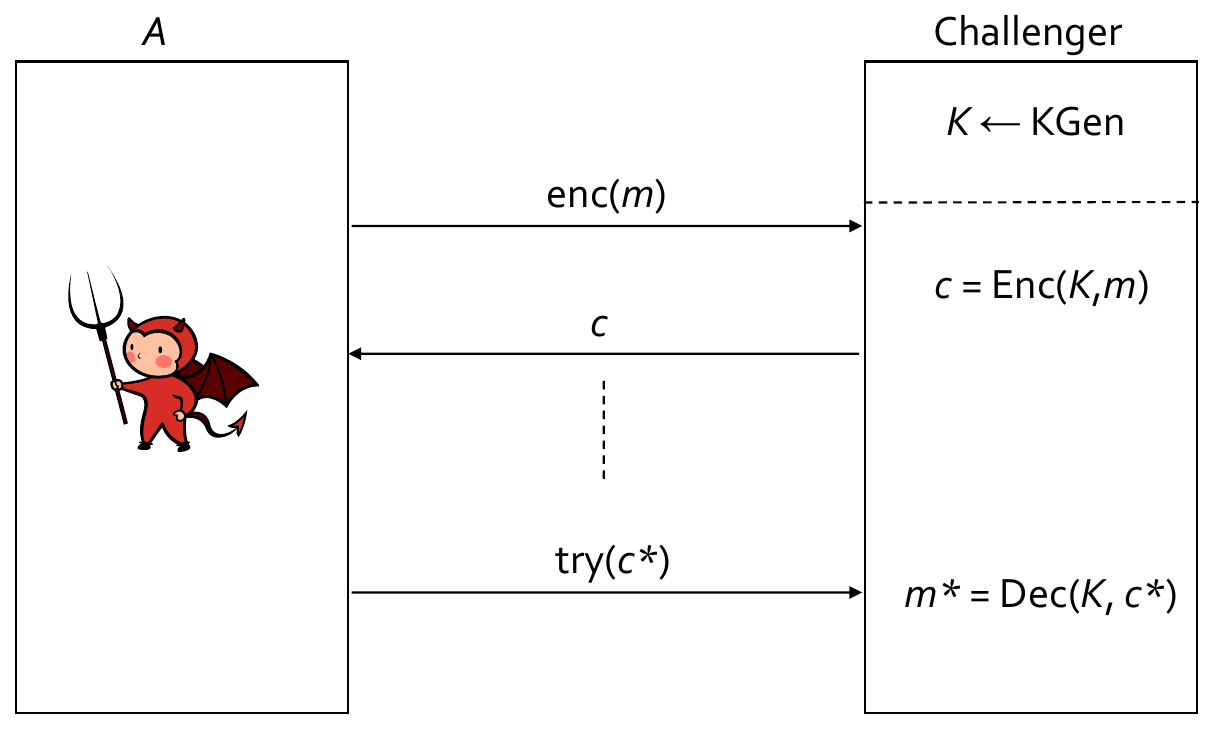
\includegraphics[scale=0.32]{images/int-ctxt-ptxt.png}
    \caption{INT-CTXT + INT-PTXT game}
    \label{fig:int-ctxt-ptxt}
\end{figure}

\paragraph{IND-CCA Security}
(Indistinguishable under chosen ciphertext attack)

Same as IND-CPA (LoR oracle), with an additional decryption oracle.%
\footnote{Trivially, the adversary is not allowed to submit ciphertexts received from the LoR oracle to the decryption oracle.}

\begin{figure}[h]
    \centering
	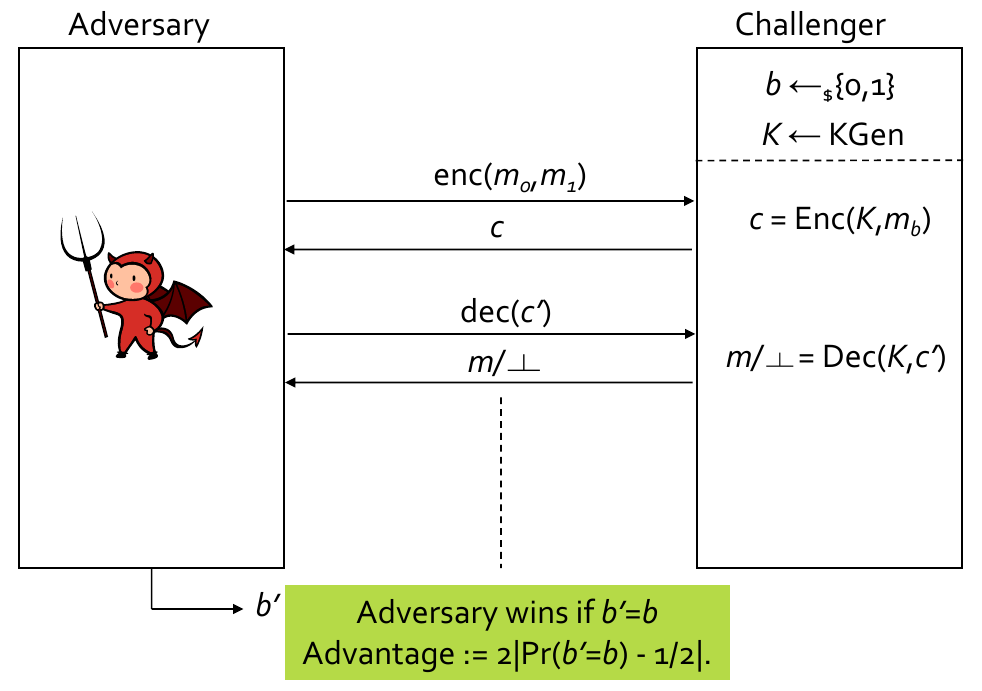
\includegraphics[scale=0.4]{images/ind-cca.png}
    \caption{IND-CCA game}
    \label{fig:ind-cca}
\end{figure}

\paragraph{Authenticated Encryption AE}
An SE is said to be \emph{AE secure} if it is IND-CPA secure and INT-CTXT secure.

AE $\implies$ IND-CCA%
\footnote{Informal proof by case distinction:
Either at some point the IND-CCA adversary queries a $c$ that does not decrypt to $\bot$ (breaking INT-CTXT) or never, in which case the decryption oracle is useless (breaking IND-CPA).
}

\paragraph{Encrypt-and-MAC E\&M}
Compute $c \leftarrow Enc_{KE}(m), \tau \leftarrow Tag_{KM}(m)$ and output $c'=c||\tau$.

NOT secure in general:
If MAC is deterministic (e.g. a PRF) then trivial IND-CPA attack applies.

E.g. in SSH (in a stateful variant).

\paragraph{Mac-then-Encrypt MtE}
Compute $\tau \leftarrow Tag_{KM}(m)$ and output $c \leftarrow Enc_{KE}(m||\tau)$.

Can be made secure under specific instantiations, but unsafe in general -- AVOID!

E.g. in TLS prior to 1.3.

\paragraph{Encrypt-then-Mac EtM}
Compute $c \leftarrow Enc_{KE}(m), \tau \leftarrow Tag_{KM}(c)$ and output $c'=c||\tau$.

AE secure under the assumption that SE is IND-CPA and MAC is \underline{S}UF-CMA.

E.g. in IPSec ESP.

\paragraph{AE with Associated Data AEAD}
Informally: integrity-protect some data, provide confidentiality for the rest.
E.g. AES-GCM, ChaCha20-Poly1305.

Both $Enc$ and $Dec$ also take the associated data $AD$ as an additional input argument
-- but the ciphertext does not ``contain'' $AD$ (instead $AD$ is sent alongside, like the nonce $N$).
\\
But: $AD$ is not an output of the AEAD scheme (only $c$ and $\tau$ are)!

IND-CPA game:
adversary sends $(N, AD, (m_0, m_1))$ to LoR oracle.

INT-CTXT game:
adversary sends $(N, AD, m)$ to encryption oracle and $(N^*, AD^*, c^*)$ to the try oracle.

EtM for AEAD:
$$
c \leftarrow Enc_{KE}(m), \tau \leftarrow Tag_{KM}(len(AD)||AD||c) ; \text{ output } c'=c||\tau
$$
Note that tagging over the length is required to avoid mis-parsing between $AD$ and $c$.

In practice:
$Enc$ and $Tag$ may be nonce-based.
If nonces implicitly use a counter, then the adversary cannot reorder or delete messages (and of course can't insert either due to INT-CTXT).

\paragraph{AES-GCM (Galois Counter Mode)}
EtM with AES in CTR mode and a CW-MAC ($H_{xpoly}$ over $GF(2^{128})$).
Single key, MAC key is derived: $K_M = AES(K, 0^{128})$.
Nonces are usually 96 bit and reuse results in catastrophic failure (MAC key recovery), thus not \emph{nonce-misuse resistant}.
Counters \underline{for $Enc$} are of the form $N||ctr$.
Almost as fast as CTR mode, since UHF in MAC is fast.

